%%%%%%%%%%%%%%%%%%%%%%%%%%%%%%%%%%%%%%%%%%%%%%%%%%%%%%%%%%%%
%%  This Beamer template was created by Cameron Bracken.
%%  Anyone can freely use or modify it for any purpose
%%  without attribution.
%%
%%  Last Modified: January 9, 2009
%%

\documentclass[xcolor=x11names,compress]{beamer}

%% General document %%%%%%%%%%%%%%%%%%%%%%%%%%%%%%%%%%
\usepackage{graphicx}
%%%%%%%%%%%%%%%%%%%%%%%%%%%%%%%%%%%%%%%%%%%%%%%%%%%%%%

%% Beamer Layout %%%%%%%%%%%%%%%%%%%%%%%%%%%%%%%%%%
\useoutertheme[subsection=false,shadow]{miniframes}
\useinnertheme{default}
\usefonttheme{serif}
\usepackage{palatino}
\setbeamerfont{title like}{shape=\scshape}
\setbeamerfont{frametitle}{shape=\scshape}

\definecolor{MpiGreen}{HTML}{007C79}
\setbeamercolor*{lower separation line head}{bg=MpiGreen} 
\setbeamercolor*{normal text}{fg=black,bg=white} 
\setbeamercolor*{alerted text}{fg=red} 
\setbeamercolor*{example text}{fg=black} 
\setbeamercolor*{structure}{fg=black} 

%%%%%%%%%%% This ugly thing disables the fading effect on block titles %%%%%%%%%%%
\pgfdeclareverticalshading[lower.bg,upper.bg]{bmb@transition}{200cm}{%
  color(0pt)=(lower.bg); color(4pt)=(lower.bg); color(4pt)=(upper.bg)}
%%%%%%%%%%%%%%%%%%%%%%%%%%%%%%%%%%%%%%%%%%%%%%%%%%%%%%%%%%%%%%%%%%%%%%%%%%%%%%%%% 

\setbeamercolor*{palette tertiary}{fg=black,bg=black!10} 
\setbeamercolor*{palette quaternary}{fg=black,bg=black!10} 

%All those fancy blocks
\setbeamertemplate{blocks}[rounded][shadow=false]
\setbeamercolor*{block title}{fg=white,bg= MpiGreen}
\setbeamercolor*{block body}{fg= black,bg= MpiGreen!10}


\newcommand{\floor}[1]{\left\lfloor #1 \right \rfloor}
\newcommand{\hlc}[1]{\textcolor{MpiGreen}{#1}}
\renewcommand{\(}{\begin{columns}}
\renewcommand{\)}{\end{columns}}
\newcommand{\<}[1]{\begin{column}{#1}}
\renewcommand{\>}{\end{column}}
%\renewcommand*\descriptionlabel[1]{\hspace\labelsep\bfseries #1}
%%%%%%%%%%%%%%%%%%%%%%%%%%%%%%%%%%%%%%%%%%%%%%%%%%
\newcommand{\abs}[1]{\vert#1\vert}
\newcommand{\eye}{\mbox{$\mbox{1}\!\mbox{l}\;$}}
%\renewcommand{\vec}[1]{\boldsymbol{#1}}
\newcommand{\herm}[1]{#1^{\dag}}
\newcommand{\vv}{\vec{v'}}

\newcommand{\be}{\begin{equation}}
\newcommand{\ee}{\end{equation}}
\newcommand{\bea}{\begin{eqnarray}}
\newcommand{\eea}{\end{eqnarray}}
\newcommand{\nn}{\nonumber}

\newcommand{\E}{{\cal E}}
\newcommand{\N}{{\cal N}}
\newcommand{\EE}{\mathbf{E}}
\newcommand{\PP}{\mathbf{P}}
\newcommand{\HH}{\mathcal{H}}
\newcommand{\F}{{\cal F}}
\newcommand{\PR}{\mathcal{PR}}

%\renewcommand{\tilde}[1]{\overset{\sim}{#1}}
\renewcommand{\tilde}[1]{\widetilde{#1}}

\graphicspath{{pics/}}
\begin{document}


%%%%%%%%%%%%%%%%%%%%%%%%%%%%%%%%%%%%%%%%%%%%%%%%%%%%%%
%%%%%%%%%%%%%%%%%%%%%%%%%%%%%%%%%%%%%%%%%%%%%%%%%%%%%%
\section{\scshape Introduction}
\begin{frame}
\title{Multistability in Kuramoto Networks}
%\subtitle{SUBTITLE}
\author{
	Debsankha Manik, Dirk Witthaut, Marc Timme
}
\date{
\begin{center}
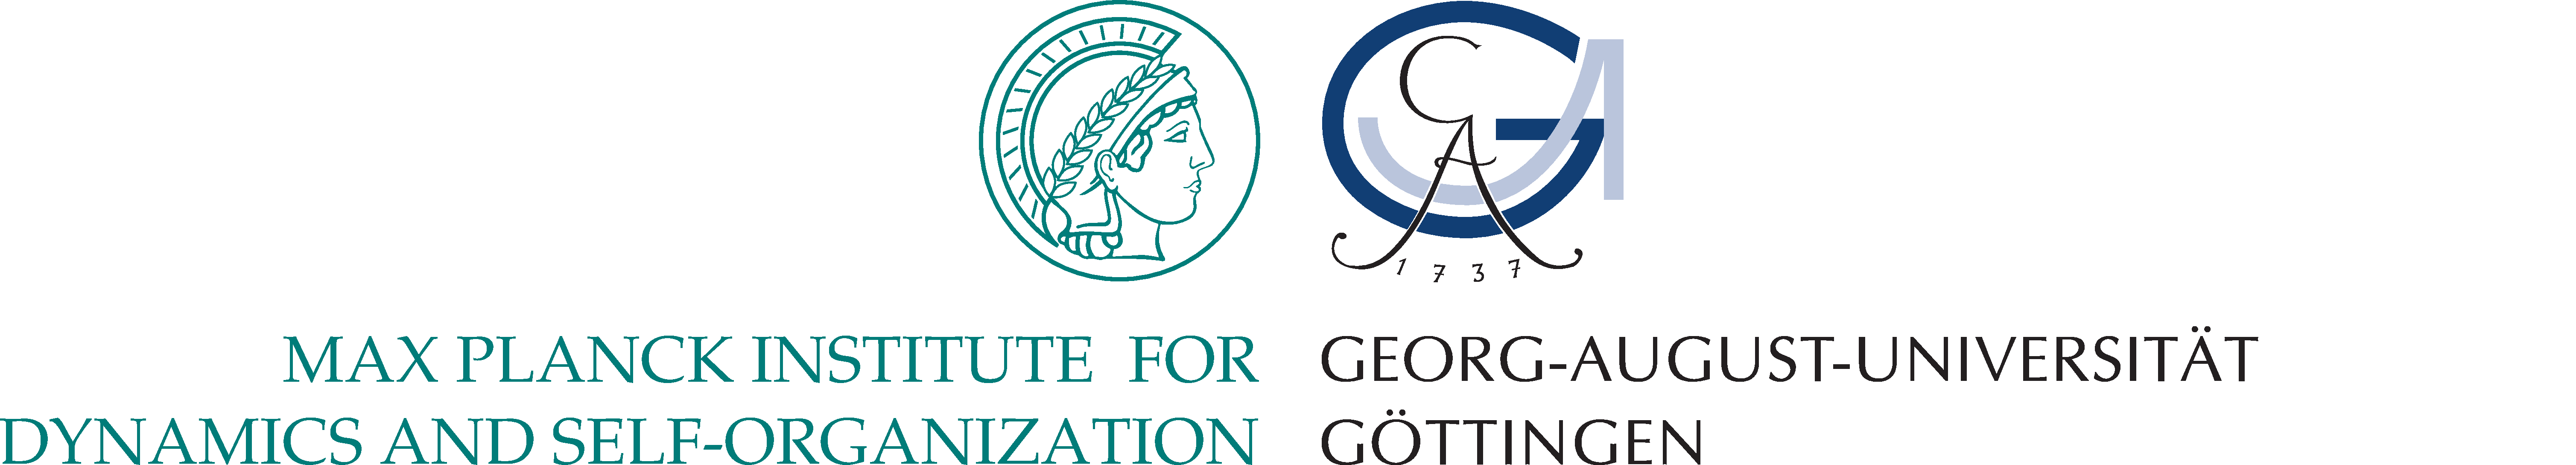
\includegraphics[width=0.9\columnwidth]{pics/dual-logo}\\
	\vspace{1cm}

\includegraphics[height=0.2\textheight]{pics/condynet_logo}
\end{center}
}
\titlepage
\end{frame}

\begin{frame}{Two models}
\begin{block}{Oscillator model for powergrid}
\begin{eqnarray*}
   \frac{d^2}{dt^2} \phi_j = P_j - \alpha  \frac{d}{dt}\phi_j
             + \sum_{\ell = 1} K _{j,\ell} \sin(\phi_\ell - \phi_j). 
  \label{eqn:power}
\end{eqnarray*}
\end{block}

\begin{block}{Kuramoto model}

\begin{eqnarray*}
   \frac{d}{dt} \phi_j = \omega_j  + \sum_{\ell = 1}^N
      K _{j,\ell} \sin(\phi_\ell - \phi_j).
   \label{eqn:kuramoto}
\end{eqnarray*}
\end{block}

Both are completely specified by the \emph{network topology} defined by the 
adjacency matrix ($K$) and the power vector ($\vec{P}$ or $\vec{\omega}$).  
\end{frame}

\begin{frame}{Fixed point}
For both the models, fixed points are the roots of this set of algebraic equations
\begin{block}{}
\begin{eqnarray*}
       P_j  + \sum_{\ell = 1}^N
      K _{j,\ell} \sin(\phi_\ell - \phi_j) =0 \qquad
     \forall j = 1,\ldots, N
    %\label{eqn:sstate}
    \label{eqn:def-steady-state}
\end{eqnarray*}
\end{block}

It is beneficial to rewrite this equation in two parts. 
\end{frame}

\begin{frame}{Part A: Dynamical condition}
\begin{block}{}
\begin{align}
   & P_j + \sum_{\ell=1}^N K _{j,\ell} S_{j,\ell} = 0 \qquad 
              \forall j=1,\ldots,N. \\
  &  |S_{j,\ell}|   \le 1 \quad \qquad \qquad \qquad  
              \forall \; \mbox{edges} \, (j,\ell).
\end{align} 
\end{block}


\begin{figure}
%\caption{}
\begin{center}
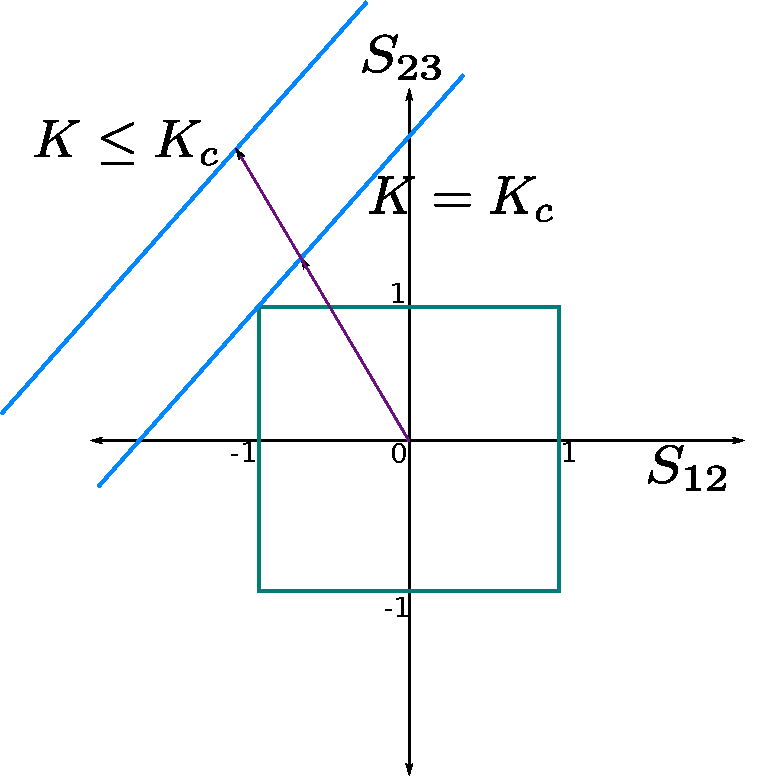
\includegraphics[height=2in]{plane-cube-intersec}
\end{center}
\end{figure}
\end{frame}


\begin{frame}{Part B: Geometric condition}
\begin{block}{}
\begin{align}
    \sum_{\rm cycle} \Delta_{j,\ell} & = 2 m \pi, \quad m\in\mathbb{Z}\\
    \Delta_{j,\ell}^+ &= \arcsin(S_{j,\ell}) \qquad \mbox{or} \\
    \Delta_{j,\ell}^- &= \pi -  \arcsin(S_{j,\ell})
     \label{eqn:deltaS} 
\end{align}
\end{block}

\begin{figure}
\begin{center}
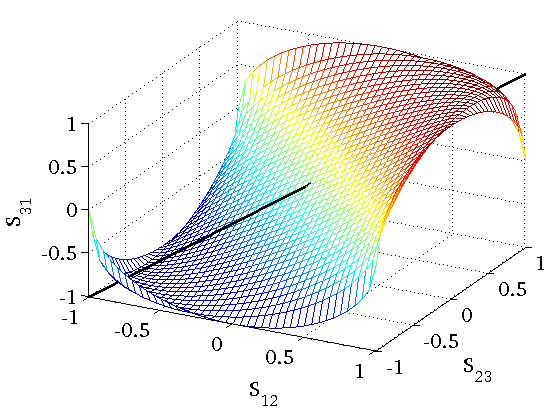
\includegraphics[width=2in]{cycle3b}
\end{center}
\end{figure}
\end{frame}

\section{Counting fixed points}
\begin{frame}{Number of fixed points in normal operation}
\begin{block}{Dynamical condition}
\begin{align}
P_j + \sum_{\ell=1}^N F_{j,\ell} &= 0 \qquad 
              \forall j=1,\ldots,N. \\
\abs{F_{j,l}}&\leq K_{j,l}
\label{eq:constraint_F}
\end{align}

\end{block}


The solutions have $\abs{E}-\abs{V}+1=\gamma$ degrees of freedom.  \\
\pause{}
Not
coincidentally, $\gamma$ is the number of basis cycles of any network.  
\end{frame}

\begin{frame}{Solution of dynamical conditions}
\begin{figure}
\begin{center}
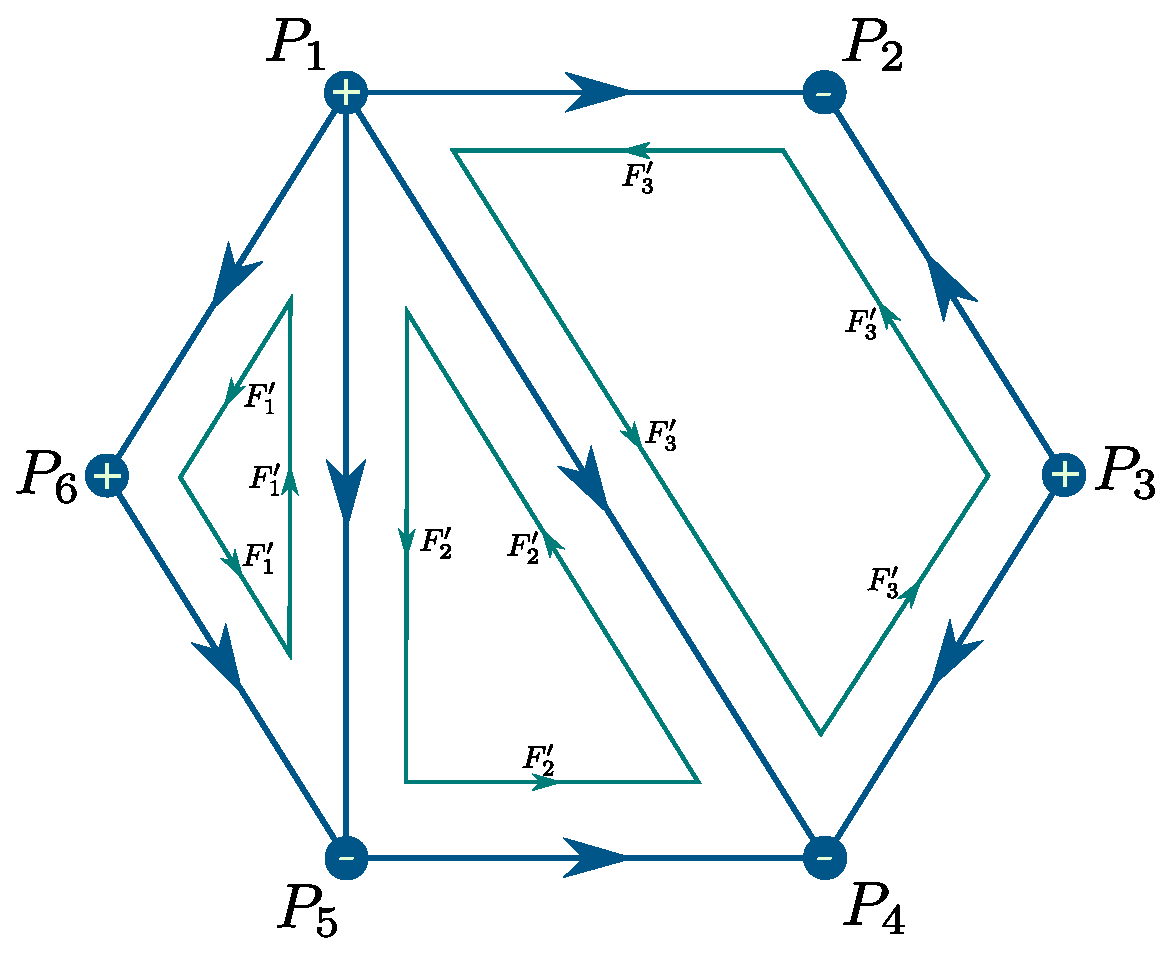
\includegraphics[width=0.7\columnwidth]{cycle_flow}
\end{center}
\end{figure}

We can add any constant flow along a \emph{cycle} subject to the constraint 
\eqref{eq:constraint_F}, and it will not violate the dynamical condition.  
\end{frame}


\section{Simple topologies}
\begin{frame}{Tree networks: no multistability}
\begin{center}
\Large{No cycleflow to add}
\end{center}
\end{frame}



\begin{frame}{Geometric condition}
\begin{block}{Discreteness in solution space}
\begin{align*}
    \sum_{\textrm{cycle k}} \arcsin(S_{j,\ell}) & = 2 \omega_{k} \pi, \quad \omega_k\in\mathbb{Z}\\
\end{align*}
\end{block}

Let's call $\omega_k\in \mathbb{Z}$ the \emph{winding number} and $\vec{\omega}:=(\omega_{1},\omega_{2},\cdots,\omega_{\gamma})$ the 
{winding vector}.  

\begin{block}{}
\begin{theorem}
\label{thm:winding}
For a planar network, corresponding to a  winding vector $\vec{\omega}$, there is either zero or one fixed point 
of the system.   
\end{theorem}
\end{block}
Therefore, number of fixed points equals the number of valid 
winding vectors. 
\end{frame}

\begin{frame}{Completely connected networks: no multistability}

\begin{block}{}
\begin{align*}
    \sum_{\textrm{cycle k}=(e_{k1}, e_{k2}, e_{k3})} \arcsin(S_{k1})+\arcsin(S_{k2})+\arcsin(S_{k3}) & = 2 \omega_{k} \pi
\end{align*}
\end{block}

Cycles has to be at least $4$ nodes big to support more than one winding 
number.  
\end{frame}






\begin{frame}{Ring networks: multistability possible}
For a homogeneous ring topology ($\left(K_{j-1,j}=K_{j,j+1}\right)$), we 
have tight bounds for the number of fixed points.  

\begin{block}{}
\begin{align}
\frac{N_c}{\pi}-\frac{N_c\bar{P}_{\max}}{2K\pi} \leq N_{f} \leq \frac{N}{2} - \frac{N_c\bar{P}_{\max}}{4K}+1.
\end{align}
\end{block}

where
\begin{align*}
N_f&=\text{number of fixed points.  }\\
N_c&=\text{number of nodes in the ring.  }\\
\bar{P}_{max}&=\text{a measure of distributiveness of the power generators}
\end{align*}

\end{frame}


\begin{frame}{Stronger coupling, distributed generators favour more fixed points}
\begin{figure}
\begin{center}
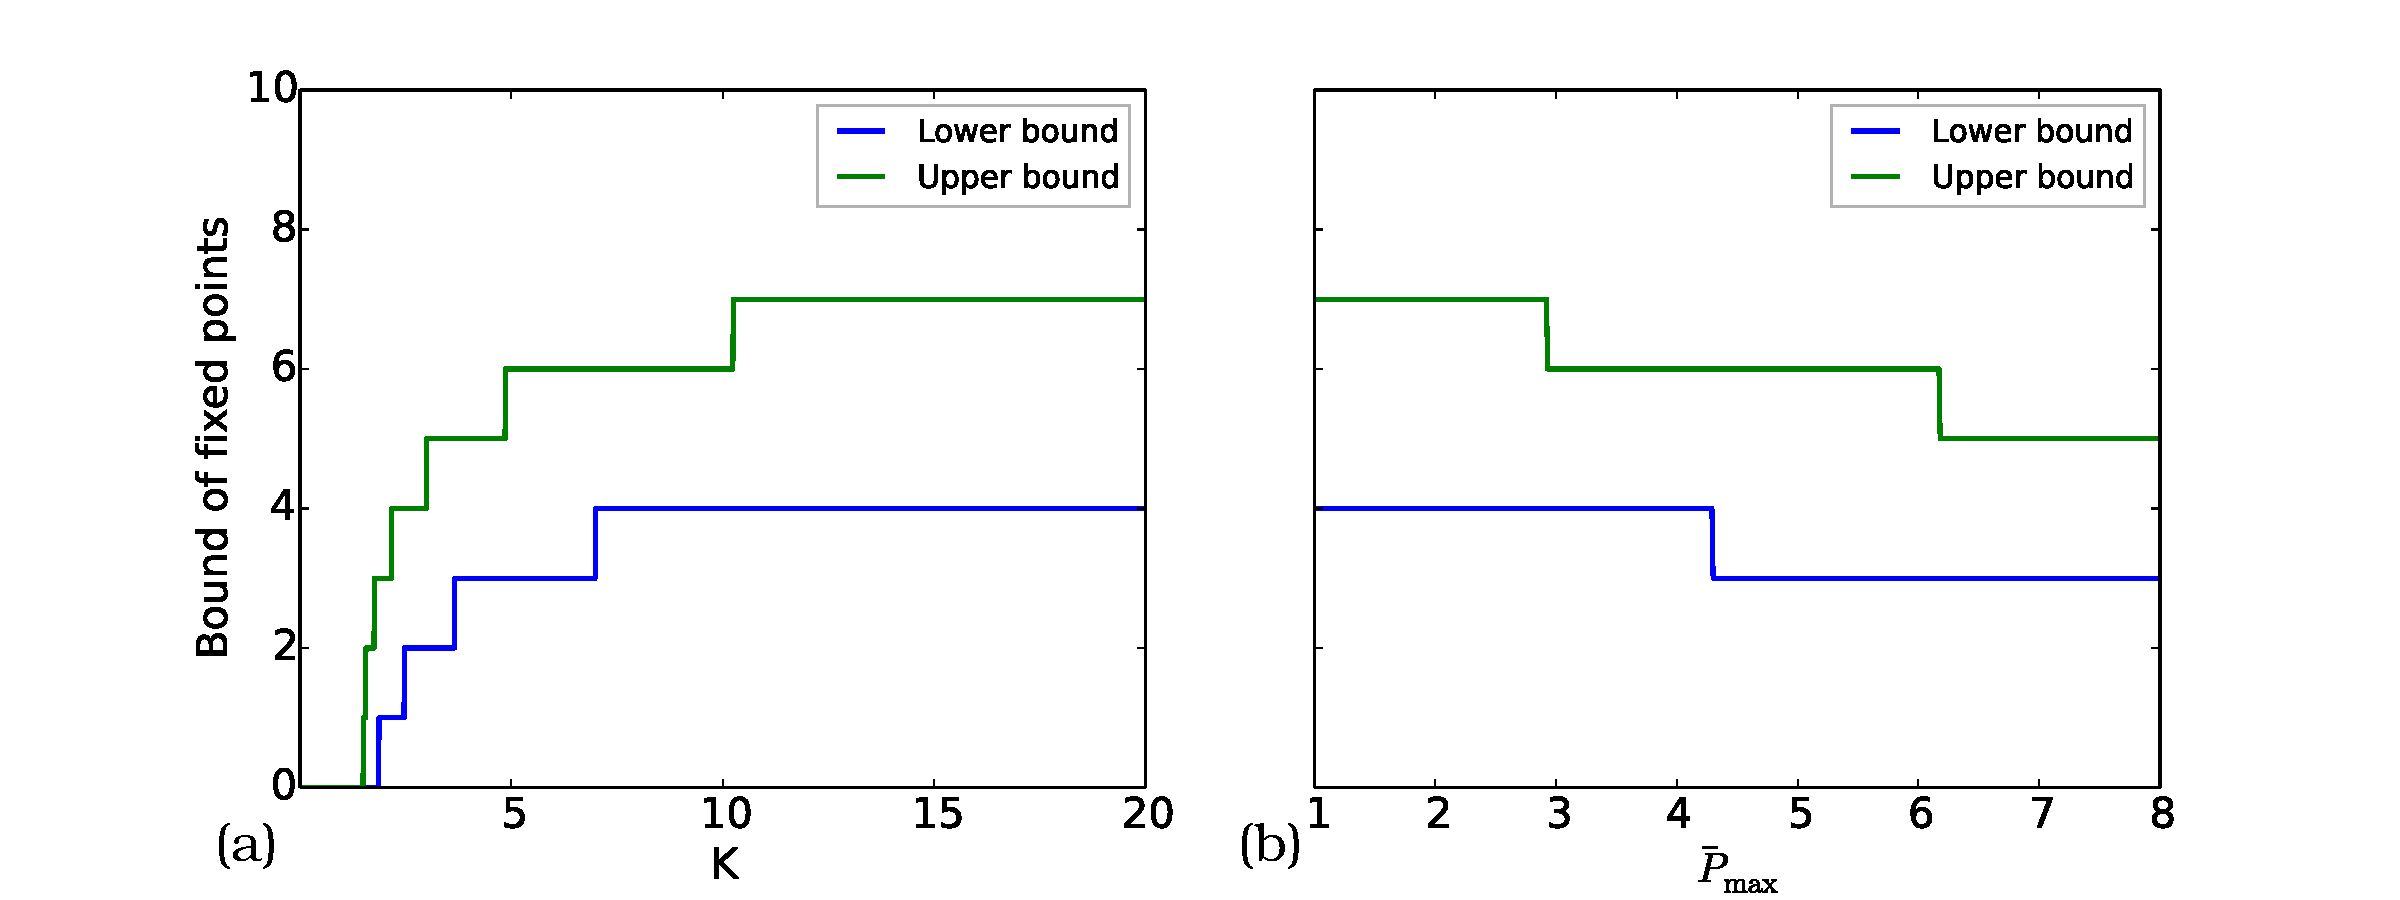
\includegraphics[width=\columnwidth]{num_fps_k_p_ring}
\end{center}
\caption{
Upper and lower bounds for the number of steady states $N_f$ 
for a sample 16 element ring as a function of (a) $K$, which is same for all 
edges, while $\bar{P}_{\max}=3$, and (b) $\bar{P}_{\max}$ while $K=10$.  
}
\end{figure}
\end{frame}





\begin{frame}{Basin volumes of fixed points}
\begin{figure}
\begin{center}
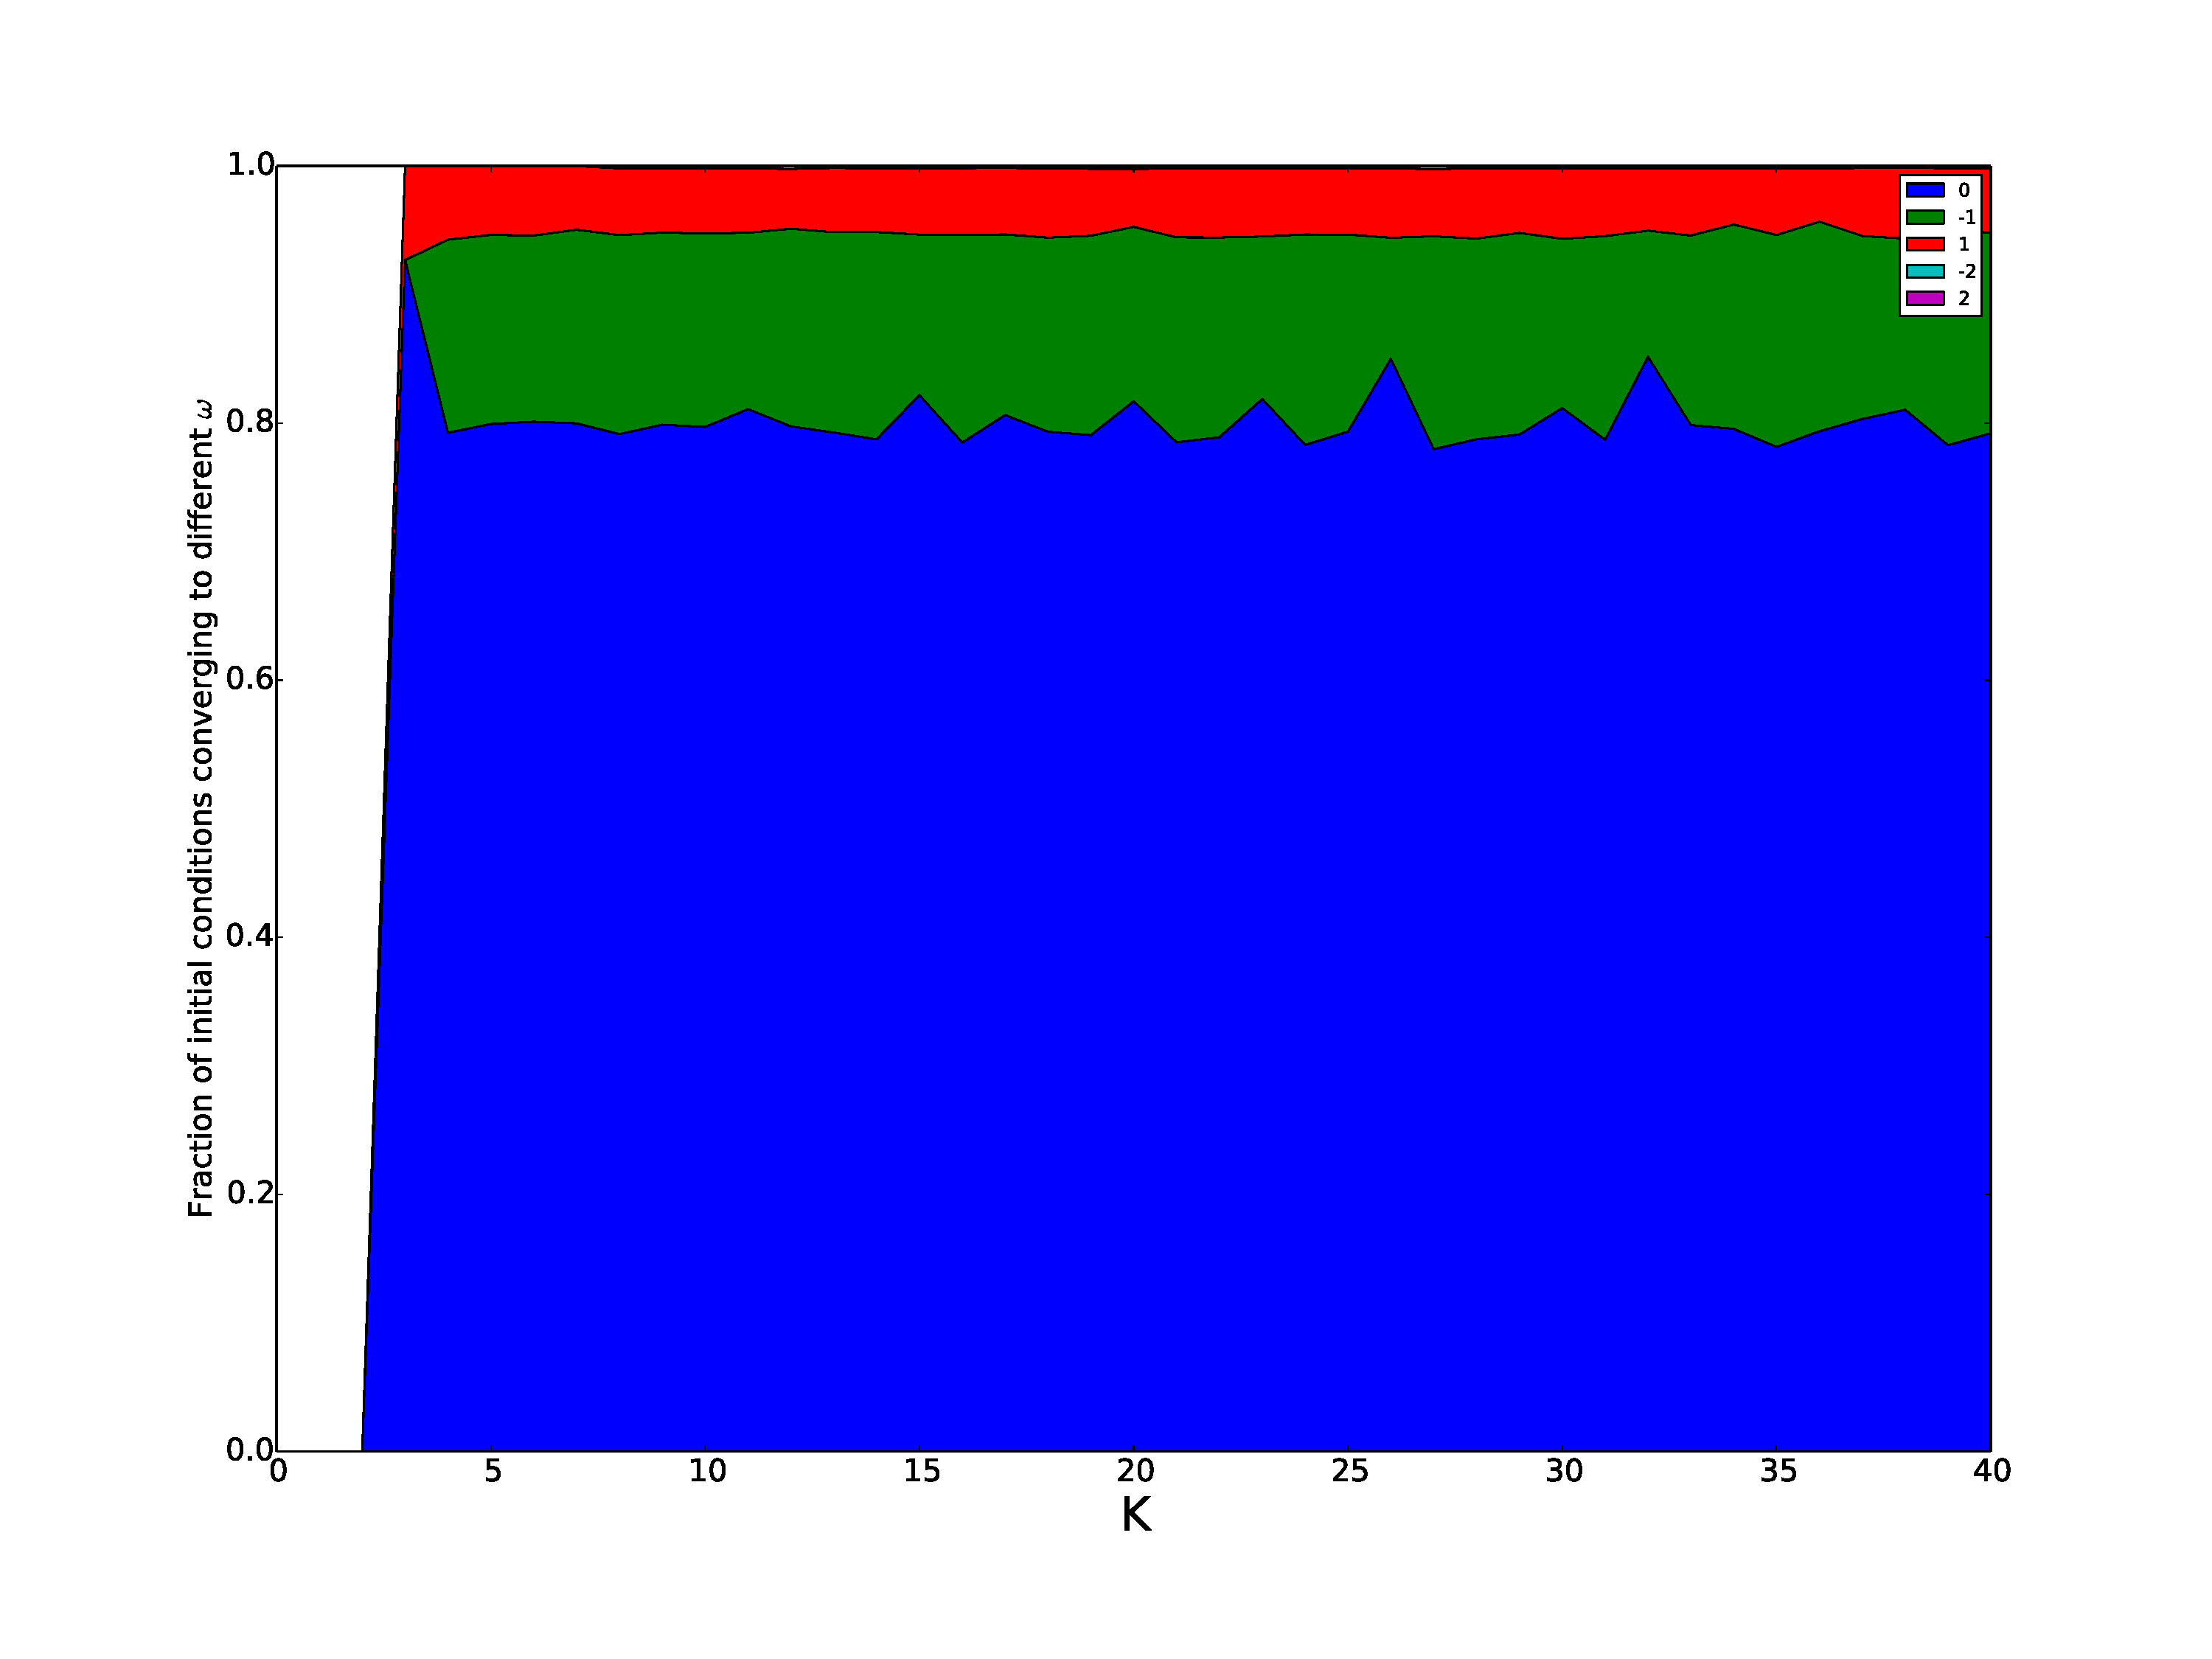
\includegraphics[width=\columnwidth]{nrepeat_20000_P_3_N_16_normcond}
\end{center}
\end{figure}

\end{frame}




\section{Arbitrary topologies}
\begin{frame}{Basin volumes for fused-ring network}
\begin{figure}
\begin{center}
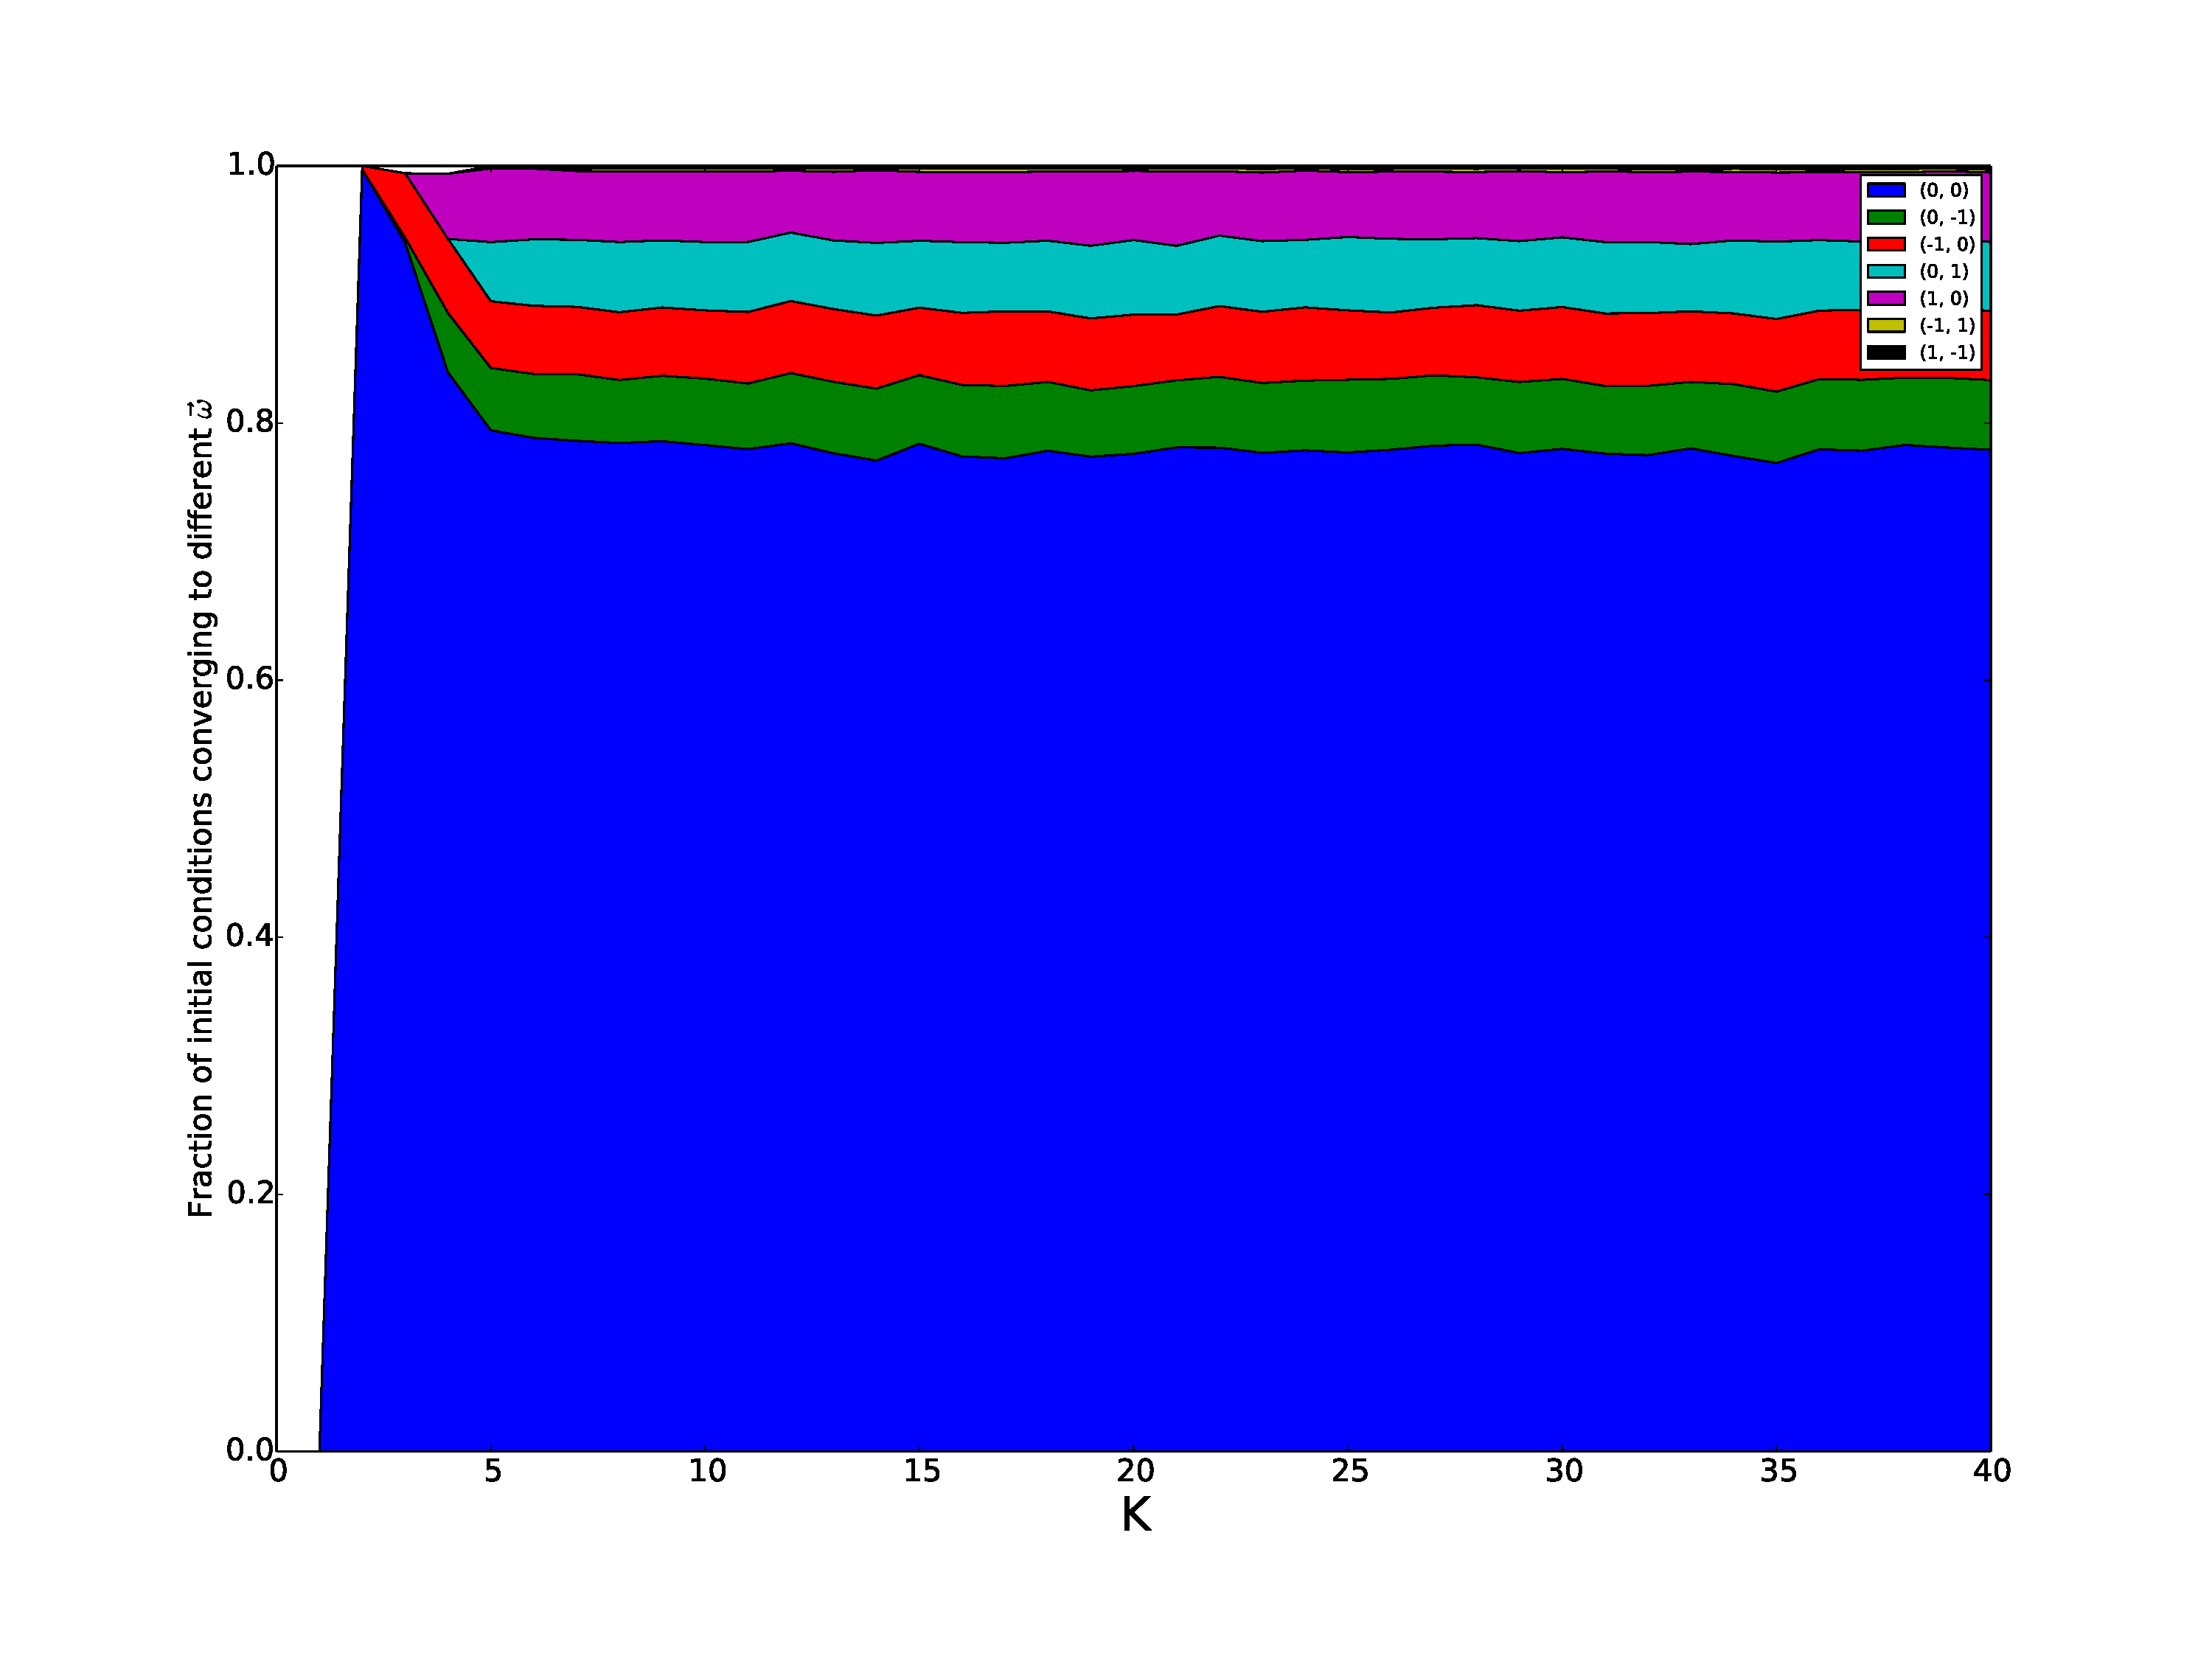
\includegraphics[width=\columnwidth]{nrepeat_20000_P_3_N_14_dualring}
\end{center}
\end{figure}

\end{frame}





\begin{frame}{Smaller loops $\Leftrightarrow$ less fixed points}

\begin{theorem}
For planar networks, the number of equilibrium states which satisfies 
$\left|\theta_i^*  - \theta_j^*\right|\leq \frac{\pi}{2}$ for all edges $(i,j)$
is bounded by
\be
   \prod_{c \in \rm{fundamental \, cycle}} \left\lfloor \frac{N_c}{2} \right \rfloor,
   \label{eqn:numsol-cycle}
\ee
\end{theorem}

\begin{figure}
\begin{center}
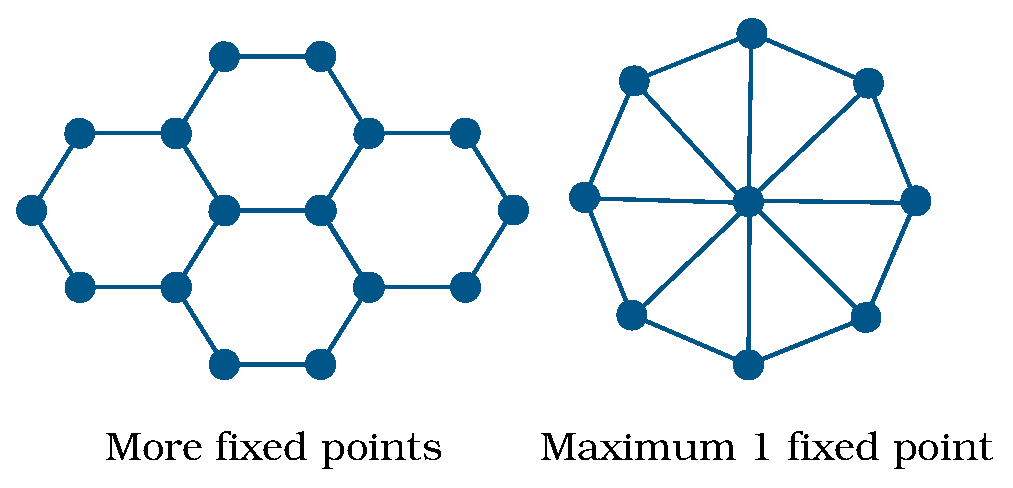
\includegraphics[width=0.8\columnwidth]{graph_faces_comp}
\end{center}
\end{figure}

\end{frame}

\begin{frame}{Critical coupling}
\begin{block}{A necessary condition}
A homogeneous Kuramoto ring will not have any fixed point unless
\[
K\geq\frac{\bar{P}_{max}}{2}
\]
\end{block}
$\bar{P}_{max}$ is the maximum (disregarding sign) power produced 
in any subset of the ring.  
\begin{figure}
\begin{center}
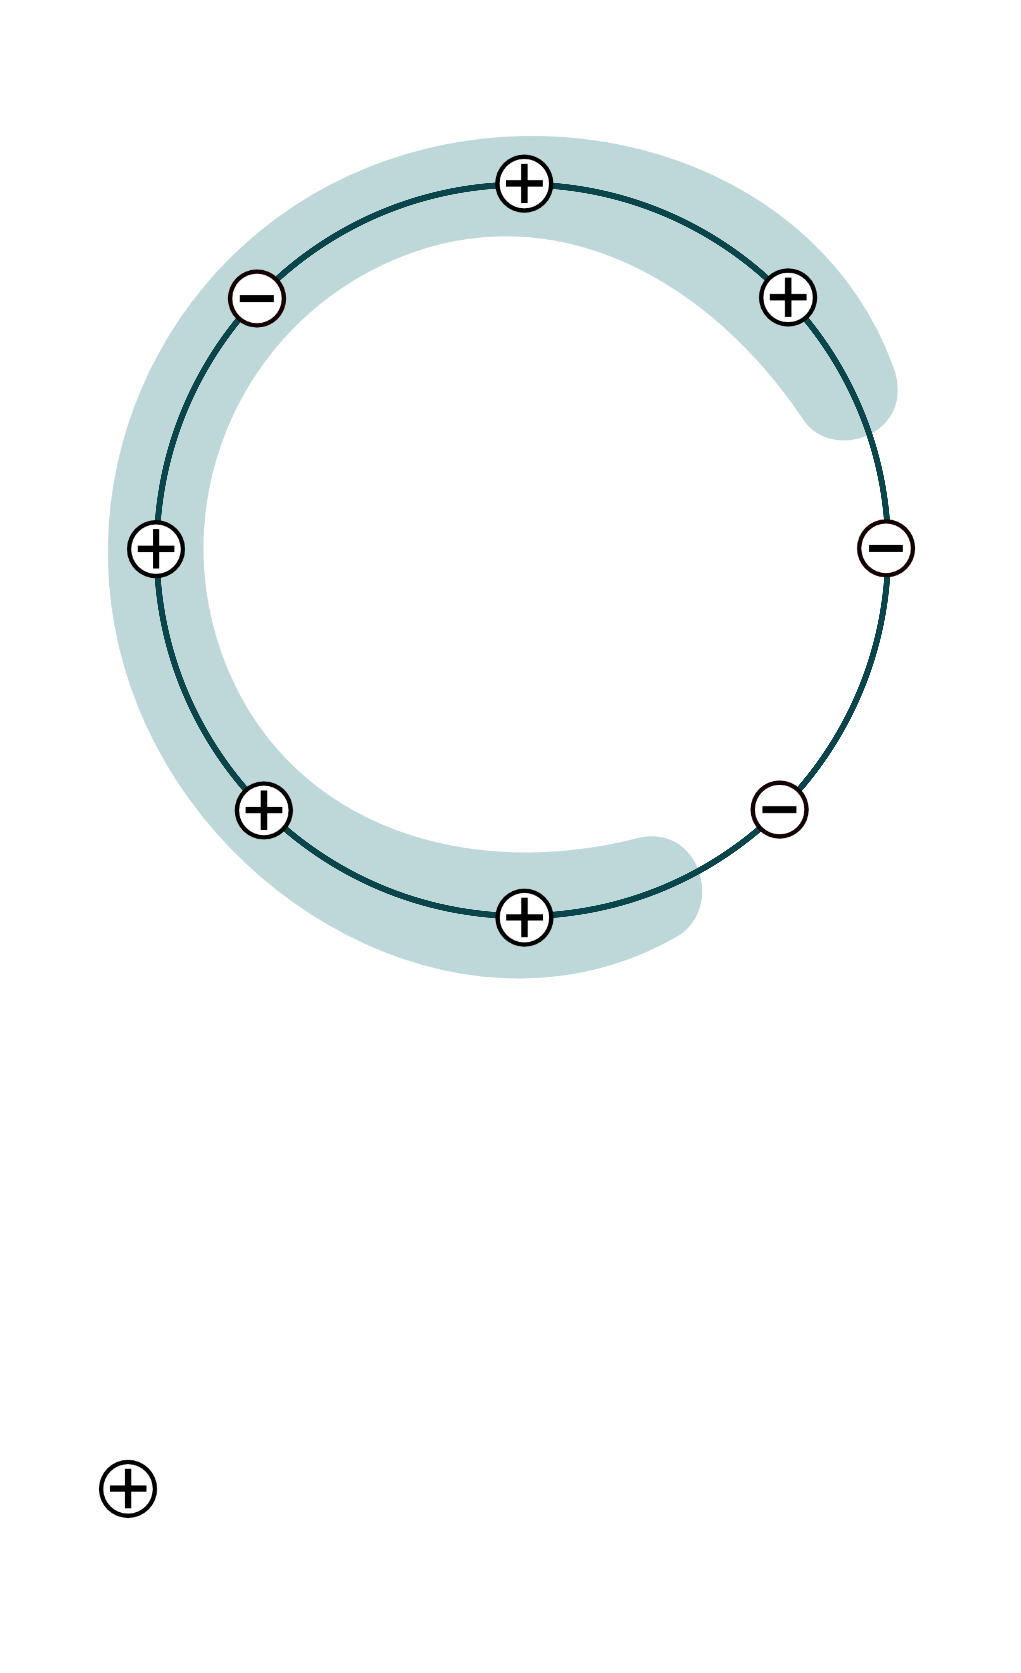
\includegraphics[width=0.3\columnwidth]{ring}
\end{center}
\end{figure}
\end{frame}

\begin{frame}{Distributed power plants $\Leftrightarrow$ less Critical 
coupling $K_c$}

\begin{figure}
\begin{center}
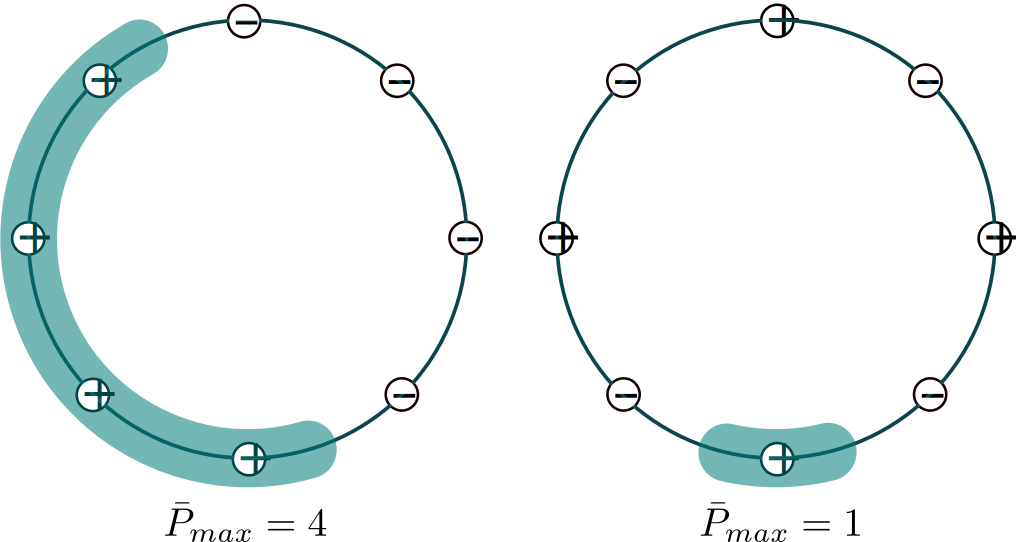
\includegraphics[width=0.9\columnwidth]{pmax_compare}
\end{center}
\end{figure}
\end{frame}


\begin{frame}{team members}
\begin{itemize}
\item Dr. Dirk Witthaut
\item Prof. Dr. Marc Timme
\item Xiaozhu Zhang
\item Benjamin Sch\"affer
\item Dr. Sarah Hallerberg
\item Dr. Nora Molkenthin
\end{itemize}

\end{frame}



\begin{frame}
\begin{center}
\Huge{\hlc{Thank You}}
\end{center}

\end{frame}





\end{document}
